\documentclass{article}
\usepackage{graphicx}
\usepackage{xcolor}
\usepackage{subcaption}
\usepackage[margin=1.0in]{geometry}
\usepackage{float}
\usepackage{ulem}
\usepackage{amsmath}
\usepackage{mathtools}
\usepackage{wrapfig}

\begin{document}
\section{Introduction}
A core problem of condensed matter physics is understanding how to systematically develop low-energy effective models for strongly correlated electron systems. In the forefront of modern research are high temperature superconductors, heavy fermion materials, materials with strong spin-orbit coupling effects, and more for which simple effective theories have not yet been found. For example, cuprate family of high-Tc superconductors have an intricate phase diagram in the doping-temperature space \textbf{ref} with a robust anti-ferromagnetic (AFM) charge-transfer insulator state near zero doping, a prominent superconducting dome in the 0.1 - 0.2 hole doped region at low temperatures with psuedo-gap and non-Fermi liquid metallic phases at higher temperatures and Fermi liquid like behavior in the overdoped area, of which only the AFM insulating and Fermi liquid phases have well understood mechanism and models \textbf{ref}. The iron-pnictides also have superconducting domes, non-Fermi liquid like metallic phases, a spin-density-wave antiferommagnetic phase, all under various dopings and temperatures \textbf{ref}. As in the cuprate case, models for these phases have not been fully fleshed out \textbf{ref}. Heavy-fermion materials have a purported quantum critical point between an AFM and Fermi-liquid phase which houses a superconducting dome, leading to another phase diagram for which building model Hamiltonians is very challenging \textbf{ref}. Materials with strong spin-orbit coupling effects exhibit a host of properties like \textbf{LIST THESE HERE!}. 

The fundamental barrier in writing down low-energy theories for strong correlated materials is the existence of non-perturbative interactions between various degrees of freedom - for example, lattice, spin and charge. Consider just the cuprate case for now, the two phases which are well understood contain a singular important degree of freedom in the low-energy space. Near zero doping the cuprates are charge-transfer insulators with an optical gap around 2 eV \textbf{ref}, indicating that the lowest energy excitations are primarily spin-like, allowing for a simple nearest-neighbor spin-only model like an AFM Heisenberg model to describe the low-energy physics quite accurately. In the heavily overdoped side, the lowest energy excitations look like well defined Fermi-liquid quasiparticles \textbf{ref}, indicating our lowest energy excitations are electron-like, and a simple non-interacting electron model (with renormalized masses, etc) will suffice. In the intermediate doping region where the low-energy excitations cannot be easily sectioned into spin-like or electron-like only, we see the emergence of exotic phases and where most difficulties arise in writing down low-energy effective models. On top of that, this entire discussion did not include any lattice effects like structural phase transitions which many strongly-correlated materials have as well \textbf{ref}.

\textbf{Current state of the art.}

We propose using a density matrix downfolding (DMD) procedure\textbf{ref} to systematically develop low-energy effective theories of the 1-band nearest-neighbor Hubbard model on a square lattice as a stepping stone towards building effective theories for strongly correlated materials. The Hubbard model is a simple model with nearest-neighbor hopping and a local on-site Coulomb repulsion, parameterized by a single ratio U/t: 
\begin{equation}
H_\text{hub} = -t \sum_{\langle i,j \rangle,\sigma}( c_{i^\dagger,\sigma} c_{j,\sigma} + h.c.) + U \sum_i n_{i\uparrow} n_{i\downarrow}
\label{hubbard}.
\end{equation}
The solutions in 1-d are well understood via the Bethe ansatz \textbf{ref}, however the 2-d square lattice Hubbard model has no known exact solution.  In the very strong coupling limit $U/t \rightarrow \infty$ an emergent low-energy spin-space exists with an effective nearest-neighbor AFM Heisenberg Hamiltonian \textbf{ref}. In the region $U = 0$ a trivial non-interacting theory holds. Between these two limits, in particular the intermediate coupling region $1 < U < 7$, no well established effective theory exists. In this region there is a metal-insulator transition at $U_c/t \sim 4$ \textbf{ref}, and the pseudogap opens up at finite temperature around $U/t \sim 7$, leading to the development of a Mott gap for large $U/t > 11$ \textbf{ref}. In addition to the half-filling phase diagram, this model exhibits a plethora of interesting ground state properties when doped including stripe phases and d-wave pairing \textbf{ref}. The relative simplicity of the Hubbard model and the lack of a well-established low-energy theory in a broad intermediate coupling region lends the model as a useful playground for our new downfolding procedure in preparation for tackling realistic strongly correlated electron systems. 

The DMD procedure allows us to develop low-energy effective theories for physical systems in a systematic manner beginning with the \textit{ab-initio} Hamiltonian:
\begin{equation}
\hat{H}_\text{ab} = -\frac{1}{2} \sum_{i} \nabla_i^2 - \sum_{i,I}\frac{Z}{|r_i - R_I|} + \sum_{i<j}\frac{1}{|r_i - r_j|}
\label{eq:Hab}
\end{equation}
where $i$ indicates electrons and $I$ nuclei, and the unit of energy is Hartree (Ha).
In this paper we will be working under the Born-Oppenheimer approximation and core electrons will be treated using pseudo-potentials.
The procedure defines a method for downfolding the \textit{ab-initio} energy functional and Hilbert space onto an effective energy functional defined on a low-energy subspace of the Hilbert space 
\begin{equation}
(E_\text{ab}, \mathcal{H}) \xrightarrow{\text{DMD}} (E_\text{eff}, \mathcal{LE} \subset \mathcal{H}), \text{ s.t. }
\forall |\Psi\rangle \in \mathcal{LE}, \ E_\text{eff}[\Psi] - E_\text{ab}[\Psi] = \epsilon[\Psi] + E_0.
\label{eq:DMD}
\end{equation} 
The energy functionals can be written as expectations over Hamiltonian operators $E_\text{ab} = \langle \Psi | \hat{H}_\text{ab} |\Psi \rangle$, $E_\text{eff} = \langle \Psi | \hat{H}_\text{eff} |\Psi \rangle$, $\epsilon$ represents the error in our effective theory, and $E_0$ is a constant energy shift.
Broadly the DMD method consists of four steps which will be discussed in detail later: 
A) Defining the space of low-energy excitations which $E_\text{eff}$ should be able to describe accurately.
B) Sampling, at minimum, a set of states in $\mathcal{H}$ which probe the chosen low-energy excitations in a statistically independent manner. The selected states need not be eigenstates. 
C) Constructing a set of candidate models which are linear in reduced density matrix (RDM) descriptors with variable coefficients $\{c\}$
\begin{equation}
E_\text{eff} = \sum_k c_k \langle \Psi | \hat{d}_k |\Psi \rangle + E_0.
\label{eq:Eeff}
\end{equation}
Here $\hat{d}_k$ are Hermitian operators typically composed of 1- or 2-RDM elements. 
Examples of possible $\hat{d}_k$ are number operators $\hat{n}_i$ and exchange operators $\vec{S}_i \cdot \vec{S}_j$.
Additionally, a single particle basis must be built to express RDM elements on and should be chosen such that variations among states in $\mathcal{LE}$ are mostly described by variations in the projection of these states onto the basis.
D) Using the samples to fit the coefficients $\{c\}$ by linear regression such that $E_\text{eff}$ satisfies the conditions in \eqref{eq:DMD} with the smallest error $\epsilon$ possible. 
The fitting procedure is typically an ordinary linear regression, however, one may use a custom cost function in the regression as well. 
In order to conduct the linear regression for a functional like \eqref{eq:Eeff}, one needs to calculate for each state sampled from $\mathcal{LE}$ the expectation values of $\hat{H}_\text{ab}$ and every descriptor $\{\hat{d}_k\}$ used in the regression.
In principle, if conducted with no approximations, the DMD method is rigorously guaranteed to obtain exact results, namely $\epsilon[\Psi] = 0$.

When downfolding $\hat{H}_\text{ab}$ we will use FN-DMC to access states in $\mathcal{LE}$ and accurately calculate their \textit{ab-initio} energies and RDM elements.
Diffusion Monte Carlo (DMC) is a quantum Monte Carlo method which projects out the ground state of a Hamiltonian given some initial trial wave function.
Consider a trial wave function $|\Psi_T\rangle$ and the Hamiltonian $\hat{H}_\text{ab}$ with ground state $|\Phi_0\rangle$. We apply the projector $e^{-\tau \hat{H}_\text{ab}}$ as $\tau \rightarrow \infty$ to $|\Psi_T \rangle$
\begin{equation}
\lim_{\tau \rightarrow \infty} e^{-\tau \hat{H}_\text{ab}} |\Psi_T\rangle 
\equiv \lim_{\tau \rightarrow \infty} |\Psi_\text{DMC}(\tau)\rangle \propto \langle \Phi_0|\Psi_T\rangle |\Phi_0\rangle,
\end{equation}
projecting out the ground state as long as the trial wave function we choose is not orthogonal to the ground state. 
The stochastic implementation involves moving samples from the trial function $\Psi_T(R)$ using the Green function $G(R, R^\prime, \tau) = \langle R | e^{-\tau(\hat{H}_\text{ab} - E_T)} | R^\prime \rangle$. Since $H_\text{ab} = T + V$, kinetic and potential energy terms, the Green function is approximated by a Trotter expansion $G(R, R^\prime, \tau) = \langle R | e^{-\tau(\hat{H} - E_T)} | R^\prime \rangle \sim \Big[e^{-d\tau(V(R) + V(R^\prime))/2} \langle R| e^{-d\tau(\hat{T} - E_T)}|R^\prime \rangle + O(d\tau^2) \Big]^N $ where $d\tau = \tau/N$.
This expansion can be interpreted as an interative procedure where samples are moved N times with a small timestep $d\tau$ until convergence.
The constant $E_T$ is a trial energy used to control the normalization of $\Psi_\text{DMC}(\tau, R)$ and is updated at each move.
This implementation, however, suffers from a fermion sign problem. 
We deal with this sign problem through a fixed-node approximation, where the nodal surface of $\Psi_\text{DMC}(\tau, R)$ is forced to match that of the initial trial wave function for all $\tau$.
This approximation makes FN-DMC variational, and will only return the exact ground state of $\hat{H}_\text{ab}$ if the nodal surfaces of $|\Psi_T\rangle$ and $|\Phi_0\rangle$ are identical.
We make use of this variational principle to access low-energy states within $\mathcal{H}$ by choosing trial wave functions with nodes that differ from the nodes of $|\Phi_0 \rangle$.
To calculate the expectation value of an operator $\hat{A}$ in FN-DMC we will use a mixed estimator $\langle \Psi_{DMC}(\tau) |\hat{A} | \Psi_T \rangle/\langle \Psi_\text{DMC}(\tau) | \Psi_T \rangle$ which allows us to use the importance sampled distribution $f = \Psi_\text{DMC}(\tau)\Psi_T$ for our Monte Carlo estimates.
Details for calculating reduced density matrix elements in FN-DMC can be found in Wagner.

\pagebreak
\section{Preliminary Work}
\subsection{Non-orthogonal determinants in FN-DMC trial wave functions}
In order to become acquainted with our code QWalk \cite{WAGNER20093390} and QMC algorithms in general I worked on implementing and testing multi-Slater-Jastrow trial functions with optimized non-orthogonal determinants (MSJ+NO) in FN-DMC \cite{Pathak2018}.
We assessed the efficiency and compactness of this new trial function by calculating the ground state energy and single particle densities of a C$_2$ molecule using FN-DMC and comparing to the results when using multi-Slater-Jastrow trial functions with optimized orthogonal determinant trial functions (MSJ+O). 
The workflow involved constructing the un-optimized trial wave functions, optimizing the parameters using an energy optimization method \cite{Toulouse2007}, and finally using the optimized trial functions in an FN-DMC calculation. 
We found that the FN-DMC energy calculated using an MSJ+NO trial function with only 24 determinants was lower than the FN-DMC energy using an MSJ+O trial function with 55 determinants. 
Further, the FN-DMC charge density calculated using MSJ+NO trial functions had stronger bonding character than when using MSJ+O trial functions, a reasonable result as introducing correlations into trial functions allows for electrons to avoid each other while still occupying the same bonding region. 
Our results indicated that using non-orthogonal determinants may lead to more compact multi-Slater-Jastrow trial wave functions for small molecules.

\subsection{Effective theory for CuO molecule using DMD}
As a first step towards developing accurate models for extended systems like solids using DMD, we constructed a many-body effective model for the CuO molecule which accurately describes the eigenstates and spectra seen in experiment up to 2eV above the ground state.
The neutral CuO molecule has been a subject of intense theoretical and experimental study due to the complex structure of its low-energy space.
While the low-energy excitations in the doublet sector of the CuO molecule are well understood, singlet selection rules for spectroscopic measurements and the doublet ground state leave the quartet sector of excitations unexplored.
We construct our $\mathcal{LE}$ based on recent anion photoelectron spectroscopy (APES) measurements of the low-lying excited states of the nuetral CuO molecule. 
The lowest energy excitations measured, which lie below 2eV, involve primarily the O 2p$_z$, 2p$_\pi$ and Cu 4s orbitals, which are fully-filled, half-filled and empty in the ground state respectively.
Beginning at 2.2 eV are excitations which remove a single electron from the fully filled Cu 3d shell and add them to either the O 2p$_\pi$ or Cu 4s orbitals.
The neutral copper atom also carries a Hund's coupling between the d and s orbitals of about $\sim$ 0.5 eV, the effects of which would be measurable among the states in $\mathcal{LE}$ as long as states of both doublet and quartet states are included.
In order to probe all of these low-energy excitations we select a low-energy space
\begin{equation}
\mathcal{LE} = \text{Span(}\{ |\Psi \rangle | \langle \Psi | \hat{n}_{3d} | \Psi \rangle \ge 9,\ \hat{H}_\text{ab}|\Psi\rangle = E |\Psi\rangle \}\text{)}.
\label{eq:LE}
\end{equation}

Our sample space was generated by using multi-Slater-Jastrow trial wavefunctions in FN-DMC. 
In principle we could probe every low-energy excitation in $\mathcal{LE}$ in a statistically independent manner by just sampling the eigenstates within $\mathcal{LE}$ and including various non-eigenstates within $\mathcal{LE}$ as well to ensure robust statistics.
In practice we do not have access to these eigenstates and approximate methods are required to sample the low-energy space. 
Consider a trial wavefunction of the form $e^{J_i} |\text{D}_i\rangle$, where $e^{J_i}$ is a three-body Jastrow factor and $|\text{D}_i\rangle$ is a determinant of some single particle orbitals.
If the nodes of $|\text{D}_i\rangle$ are similar to the nodes of an eigenstate $|\Phi_i\rangle \in \mathcal{LE}$, then the properties and energy calculated from FN-DMC using this trial wavefunction will approximate those of the eigenstate, with the degree of approximation depending on the quality of the trial function nodal structure.
If we were able to find for each $|\Phi_i \rangle \in \mathcal{LE}$ such a $|\text{D}_i\rangle$ then we can approximate any state in $\mathcal{LE}$ as
\begin{equation}
|\Psi\rangle = \sum_i c_i |\Phi_i\rangle \sim \sum_i c_i \lim_{\tau \rightarrow \infty} e^{-\tau \hat{H}_\text{ab}} (e^{J_i} |D_i\rangle) \xrightarrow{J_i = J} \lim_{\tau \rightarrow \infty} e^{-\tau \hat{H}_\text{ab}} (e^{J}\sum_{i} c_i|\text{D}_i\rangle).
\label{eq:sampling}
\end{equation}
The last equality is valid if $\forall i\  J_i = J$, allowing us to map $|\Psi \rangle \in \mathcal{LE}$ to the end result of an FN-DMC calculation using a multi-Slater-Jastrow trial wavefunction. 
We use symmetry-targeted unrestricted Kohn-Sham (UKS) to generate our determinants $|\text{D}_i\rangle$ using a B3LYP functional, which has been shown to accurately reproduce ground state nodal properties of transition-metal oxide molecules, a Trail-Needs pseudopotential, and the VTZ Trail-Needs basis using the package PySCF.
This method allows us to access almost every excitation in $\mathcal{LE}$, however, there are some cases of two or more low-energy states within $\mathcal{LE}$ which have identical S$_z$ and number of electrons per irrep.
An example of this dilemma would be the ground state and the state with an excitation from Cu 3d$_{xz} \rightarrow $  O 2p$_x$.
In these few cases the higher energy excited $|\text{D}_i\rangle$ is inaccessible and the corresponding $|\Phi_i\rangle$ is excluded from the sum in \eqref{eq:sampling}, restricting our sample space to a subspace of $\mathcal{LE}$.
We will discuss the consequences of this restriction later on.
A single three-body Jastrow factor $J$ was used for every $|\text{D}_i\rangle$ and was optimized on the lowest energy UKS state using a linear energy optimization method.
The FN-DMC calculations were conducted with T-moves, to make the calculation variational while using pseudopotentials, with a timestep of $\tau = 0.01$.
The coefficients $\{c_j\}$ for our sample states were chosen via a shell-sampling method. 
We begin by fixing the coefficient $c_0 = \sqrt{w}$ where $w \in \{1.0, 0.8, ..., 0.2\}$. 
For each choice of $w$ we sample n = 5 states by randomly selecting the unassigned coefficients from a uniform distribution such that $\sum_i c_i^2 = 1$. 
This procedure generates shells of samples at decreasing distance from the eigenstate $|\Phi_0\rangle$. 
We can then loop over all $i$ to generate shells near each eigenstate.

Parameterizing our effective model requires constructing a basis on which to calculate our \textit{ab-initio} 1-/2-RDM elements and selecting a set of descriptors from which we would like to build our model.
We constructed two such bases: a localized intrinsic atomic orbital (IAO) basis and a molecular orbital (MO) basis.
The IAO basis was built on all Cu 3d, 4s and O 2p molecular orbitals from the $|\text{D}_i\rangle$ used to construct our sample states.
The MO basis consists of the Cu 3d, 4s and O 2p molecular orbitals from the lowest energy restricted open-shell Kohn-Sham (ROKS) solution with $x \leftrightarrow y$ spatial symmetry, a O 2p$_z \rightarrow$ O 2p$_\pi$ excitation.
We determine whether each basis is valid by looking at how much the trace of 1-RDM in FN-DMC on that basis differs from the expected value of 15 electrons.
We find that within 95\% confidence the trace is 14.7-14.8 (MO) and 14.6 - 14.7 (IAO), indicating that the major variation between states in $\mathcal{LE}$ can be described by either single particle basis.
As these two bases are used to describe the same space, they are related by a  transformation which will allow us to map between them if necessary.
As these two bases are used to describe the same space, they are related by an orthogonal transformation which will allow us to map between them if necessary.
In order to describe the low-energy degrees of freedom in the CuO molecule our model will require occupation energies and hybridizations between the Cu 3d, 4s and O 2p atomic orbitals which are most compactly represented in an MO basis.
The lack of doubly occupied Cu 4s states in the low-energy spectrum of CuO indicate the necessity of a Hubbard U term on the Cu 4s.
This is corroborated by the fact that the FN-DMC energy of the lowest-lying sampled state with a doubly occupied Cu 4s orbital is 7 eV above the lowest energy sampled state.
Further, we include a Hund's coupling between the Cu 4s and Cu 3d orbitals in our model based on the existence of a similar Hund's coupling 
for the copper atom.
These two interaction terms are best represented in the IAO basis as they are intuitively interactions between localized orbitals.
In addition to these important parameters, we will consider models which contain any number of hybridizations between the MOs to account for orbital relaxation between excited states in the CuO molecule.
In total our space of canditate models is then 
\begin{equation}
\begin{split}
\{\bar{n}_{4s}, \bar{n}_{p_\pi}, \bar{n}_{p_z}, \hat{n}_{4s\uparrow} \hat{n}_{4s\downarrow},\sum_{i \in \{xy, xz, ...\}}\vec{S}_{4s}\cdot \vec{S}_{d_i}\} \ + \\
\text{P}(\bar{c}_{d_\pi}^\dagger \bar{c}_{p_\pi} + h.c.,\ \bar{c}_{d_z^2}^\dagger \bar{c}_{p_z} + h.c.,\ \bar{c}_{4s}^\dagger \bar{c}_{p_z} + h.c.,\ \bar{c}_{d_z^2}^\dagger \bar{c}_{4s} + h.c.)
\end{split}
\label{eq:models}
\end{equation}
where P denotes the power set and operators are defined on the IAO basis unless denoted by a bar, in which case the operator is built on the MO basis. The coefficients for each term above will be denoted $\bar{\epsilon}_{4s},\ \bar{\epsilon}_{p_\pi},\ \bar{\epsilon}_{p_z},\ U_s,\ J_{sd},\ \bar{t}_\pi,\ \bar{t}_{dz},\ \bar{t}_{sz},\ \bar{t}_{ds}$. The operator $\bar{n}_{3d}$ is not included in any models as it is linearly dependent on all other occupation energies through the relationship $\bar{n}_{3d} + \bar{n}_{p_z} + \bar{n}_{p_\pi} + \bar{n}_{4s} = N_\text{elec} = \text{15}$. The symbol $\pi$ denotes a contraction over $x, y$ for p orbitals and $xz,\ yz$ for d orbitals. The symbol $\delta$, introduced later, denotes a contraction over $xy,\ x^2-y^2$ for d orbitals.

After fitting each of the potential models in \eqref{eq:models} using ordinary linear regression (OLS) and solving the resultant models using exact diagonalization, we find a set of models which describe the energy functional on our sample set accurately but whose eigenstates and spectra differ as a consequence of intruder states below an energy of 2eV. 
The sixteen different models all regress with R$^2 >$ 0.95 on our sample data, however some models are more robust than others. 
Models which have coefficients that are zero within 95\% confidence intervals, computed through bootstrap estimates, are removed from consideration.
Any models which have an average errorbar in the first 20 exactly diagonalized eigenvalues, also estimated by bootstrapping, greater than 0.20 eV are ignored.
Each of the remaining three models describe our sample set accurately, have robust non-zero coefficients, and have small error bars in eigenvalues of states which we care about the most.
However, the eigenstates below 2eV differ greatly between these models as illustrated in Figure \ref{fig:InitED}.

\begin{figure}[H]
\begin{center}
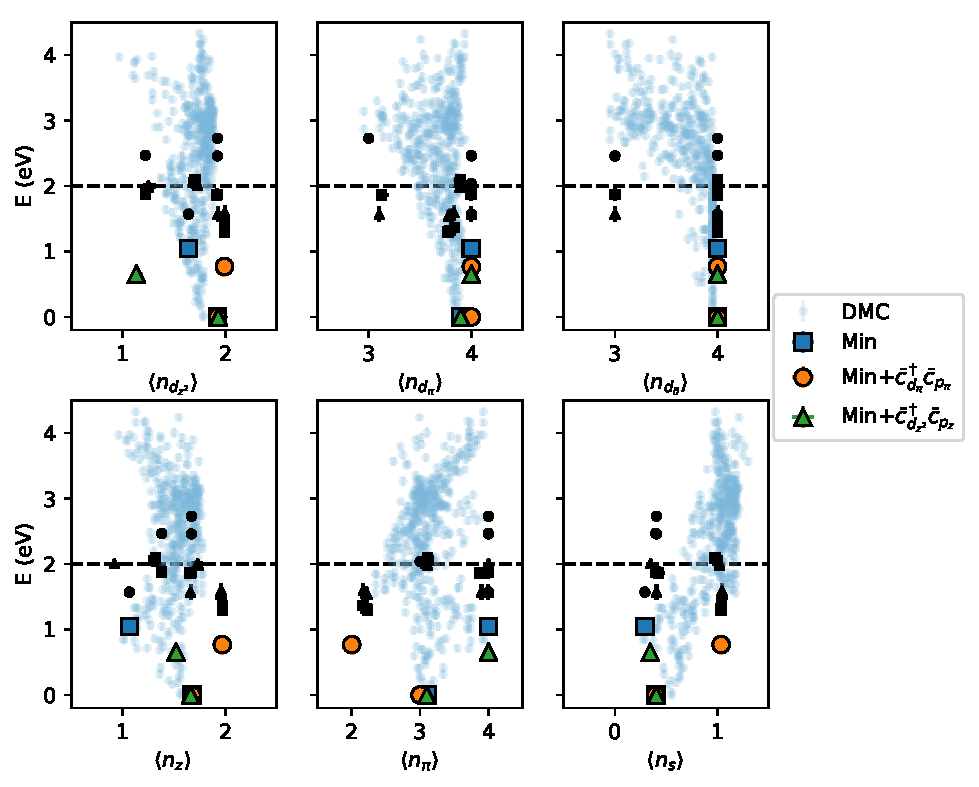
\includegraphics[width=0.7\linewidth]{../cuo/qwalk/old/ub3lyp_s1_/analysis/figs/init_ed.pdf}
\end{center}
\caption{Results of exact diagonalization showing the energies and properties of the first twenty eigenstates for three candidate models fit using ordinary linear regression. The ground state and first excited state are colored and have enlarged markers for clarity. Error bars are 95\% CI calculated by a bootstrap estimate.}
\label{fig:InitED}
\end{figure}

All three models have a first excited state around 1eV, but only in the minimal model does this state fall near the sample set used for the fitting, and is the only model in which this state corresponds to the correct excitation O 2$p_z \rightarrow $ O 2p$_\pi$ as seen in experiment.
In contrast, the first excited state for the other two models are visibly distant from our sample set and do not correspond to the experimental first excited state.
The large distance of these eigenstates from our sample set indicates that their predicted eigenvalues may suffer from large extrapolation errors, and as such we will call them \textit{intruder} states.
In Figure \ref{fig:Intruder} we present all eigenstates among the three potential models which we classify as intruders using a k-nearest neighbor approach with k = 5.

Given that our intruder states correspond to states within $\mathcal{LE}$ but outside our sample set, they must live within the span of the eigenstates which were excluded in our sampling scheme as described before.
This is evidenced by the fact that two of the intruder states correspond explicitly to excitations we could not access: Cu 3d$_{z^2} \rightarrow $ O 2p$_\pi$ and  Cu 3d$_\pi \rightarrow $ O 2p$_\pi$.
In fact, these are the only two singly excited states which we could not access with our sampling scheme.
While inaccessible, we can approximate these states by single rigid MO excitations above the UKS ground state, which results in states with a FN-DMC energy above 4eV.
Including a generous 2eV reduction in FN-DMC energy due to orbital relaxation, we estimate that these two states should lie at least 2eV in energy. 
Since all the other inaccessible eigenstates are double or higher order excitations, our very approximate exploration of the inaccessible parts of $\mathcal{LE}$ leaves us with a reasonable prior: intruder states should lie above 2eV in energy in our effective theories.
We can enforce this prior by adding a term to our ordinary linear regression cost function
\begin{equation}
\text{Cost} = \sum_{i} (E_\text{eff}[\Psi_i] - E_\text{ab}[\Psi_i])^2 + \lambda \sum_{p}\text{QHL}(2 - E_\text{eff}[\Psi_p]),\ \text{QHL}(x) = \Theta(x)x^2
\label{eq:cost}
\end{equation}
where $\lambda>0$ is a parameter which can be varied, QHL is a quadratic hinge loss, $\Theta$ is the Heaviside step function, the index $i$ is over our sampled states and $p$ over the selected intruder states.
Increasing the value of $\lambda$ leads to a stronger penalty for models which do not satisfy our prior.

\begin{figure}[H]
\begin{center}
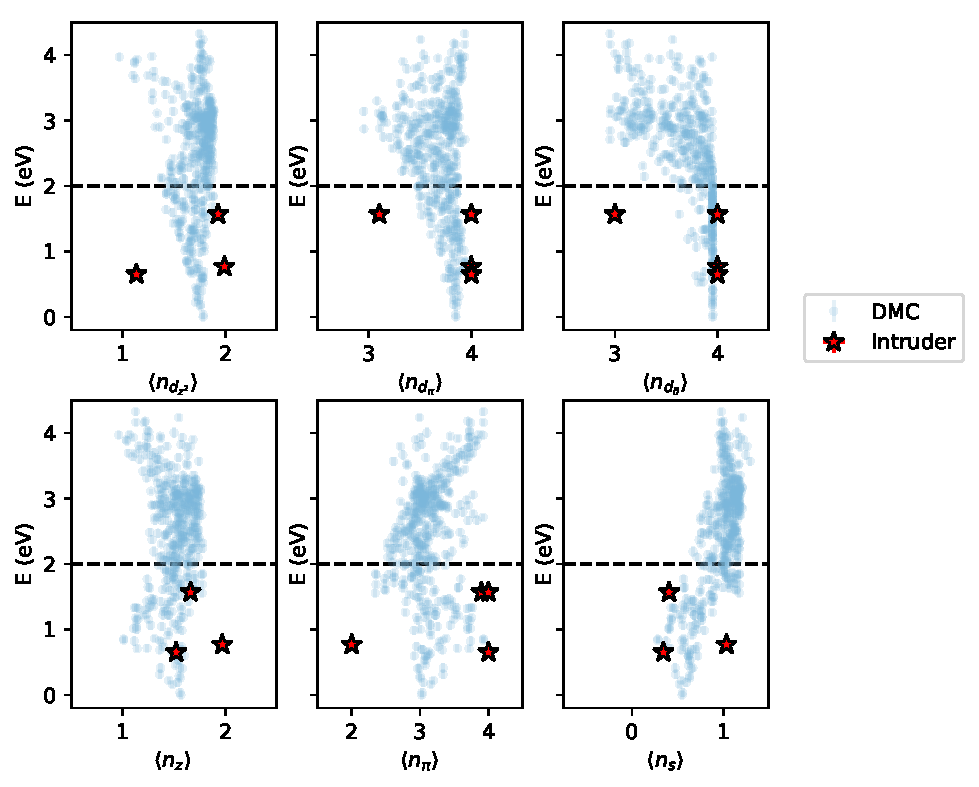
\includegraphics[width=0.7\linewidth]{../cuo/qwalk/old/ub3lyp_s1_/analysis/figs/intruder.pdf}
\end{center}
\caption{Collection of unique intruder states from our three potential models selected using a k-nearest neighbor approach with k = 5.}
\label{fig:Intruder}
\end{figure}

Using our new cost function we find a set of models which accurately describe our sample data, have very similar spectra and eigenvectors, and do not contain intruder states below the 2eV prior. 
Shown in Figure \ref{fig:Prior} are the R$^2$ scores and QHL for the three candidate models fit at $\lambda \in [0,20]$. 
The R$^2$ score stays above 0.95 for all models and $\lambda$, and the QHL converges quickly to nearly zero at $\lambda = 20$ for all three models. 
We conclude that all three models at $\lambda = 20$ should be considered good models as they satisfy our prior and also explain our sample set accurately. 
Also shown are $E_\text{eff}, E_\text{ab}$ for our samples using the minimal model at $\lambda = 20$ to illustrate the high fit quality even with a large $\lambda$.
Figure \ref{fig:FinalED} presents the properties and eigenvalues of the lowest 30 eigenstates for the three fit models at $\lambda = 20$. 
In comparison one can view Figure \ref{fig:InitED} as the same figure for fits at $\lambda = 0$. 
At $\lambda = 20$ there are no outliers below 2eV in any of the three fit models. 
The additional constraint from asserting a prior has seemingly caused a single effective theory to emerge from our set of candidate models.
This conclusion is verified by looking at the values of the fit parameters for our three models, presented in Table 1.
The parameter values for the three different models fit at $\lambda = 20$ are nearly identical within error bars and indicate that asserting our prior ensures that all candidate models regress to a single low-energy effective theory.
All occupation energies are relative to $\epsilon_{d_\delta}$.

Our final regressed model accurately reproduces properties and energies of the lowest lying eigenstates as seen in modern APES experiments on the CuO molecule.
From Figure \ref{fig:FinalED} we see that the ground state of our effective theory has fully filled Cu 3d shell, nearly two electrons in O 2p$_z$ orbital, three in the O 2p$_\pi$ and around a quarter of an electron in the Cu 4s orbital.
An approximate electronic configuration for the ground state is therefore
be assigned 1$\sigma^2$1$\pi^4$1$\delta^4$2$\sigma^2$2$\pi^3$3$\sigma^0$ where the orbitals associated with the assignment are Cu 3d$_{z^2}$, Cu 3d$_\pi$, Cu 3d$_\delta$, O 2p$_z$, O 2p$_\pi$, and Cu 4s.
This state also has a total spin projection S$_z = \frac{1}{2}$.
This matches the well studied ground state electron configuration for the molecule $^2\Pi$.
There are two excited states around 1eV in energy, the first of which is a state with the following single excitation O 2p$_z \rightarrow$ O 2p$_\pi$, has the configuration 1$\sigma^2$1$\pi^4$1$\delta^4$2$\sigma^2$2$\pi^4$4$\sigma^0$, and S$_z = \frac{1}{2}$.
According to experiment there is also such a state at 1eV and is usually denoted as $^2X$.
A second excited state at 1.2 eV exists which corresponds to an excitation 
O 2p$_\pi \rightarrow$ Cu 4s, has configuration 1$\sigma^2$1$\pi^4$1$\delta^4$2$\sigma^2$2$\pi^2$4$\sigma^1$, and can either be S$_z = \frac{1}{2}, \frac{3}{2}$. 
This is also the lowest energy eigenstate which can be a spin quartet.
\textbf{ref} agree that this excitation should be the lowest spin quartet excitation, but argue that this state should be at an energy of 1.9 eV. 
Our model has a different spin quartet state with a full Cu d shell at 1.9 eV, corresponding to an excitation O 2p$_z \rightarrow$ Cu 4s, with configuration 1$\sigma^2$1$\pi^4$1$\delta^4$2$\sigma^1$2$\pi^4$4$\sigma^1$. 
There are another host of eigenstates for our models at 2 eV corresponding to singles excitations of the form Cu 3d $\rightarrow$ O 2p$_\pi$. 
This matches measurements which indicate that the lowest energy eigenstates with a single hole in the Cu 3d shell lie at 2.2 eV above the ground state.


\begin{figure}[H]
\begin{center}
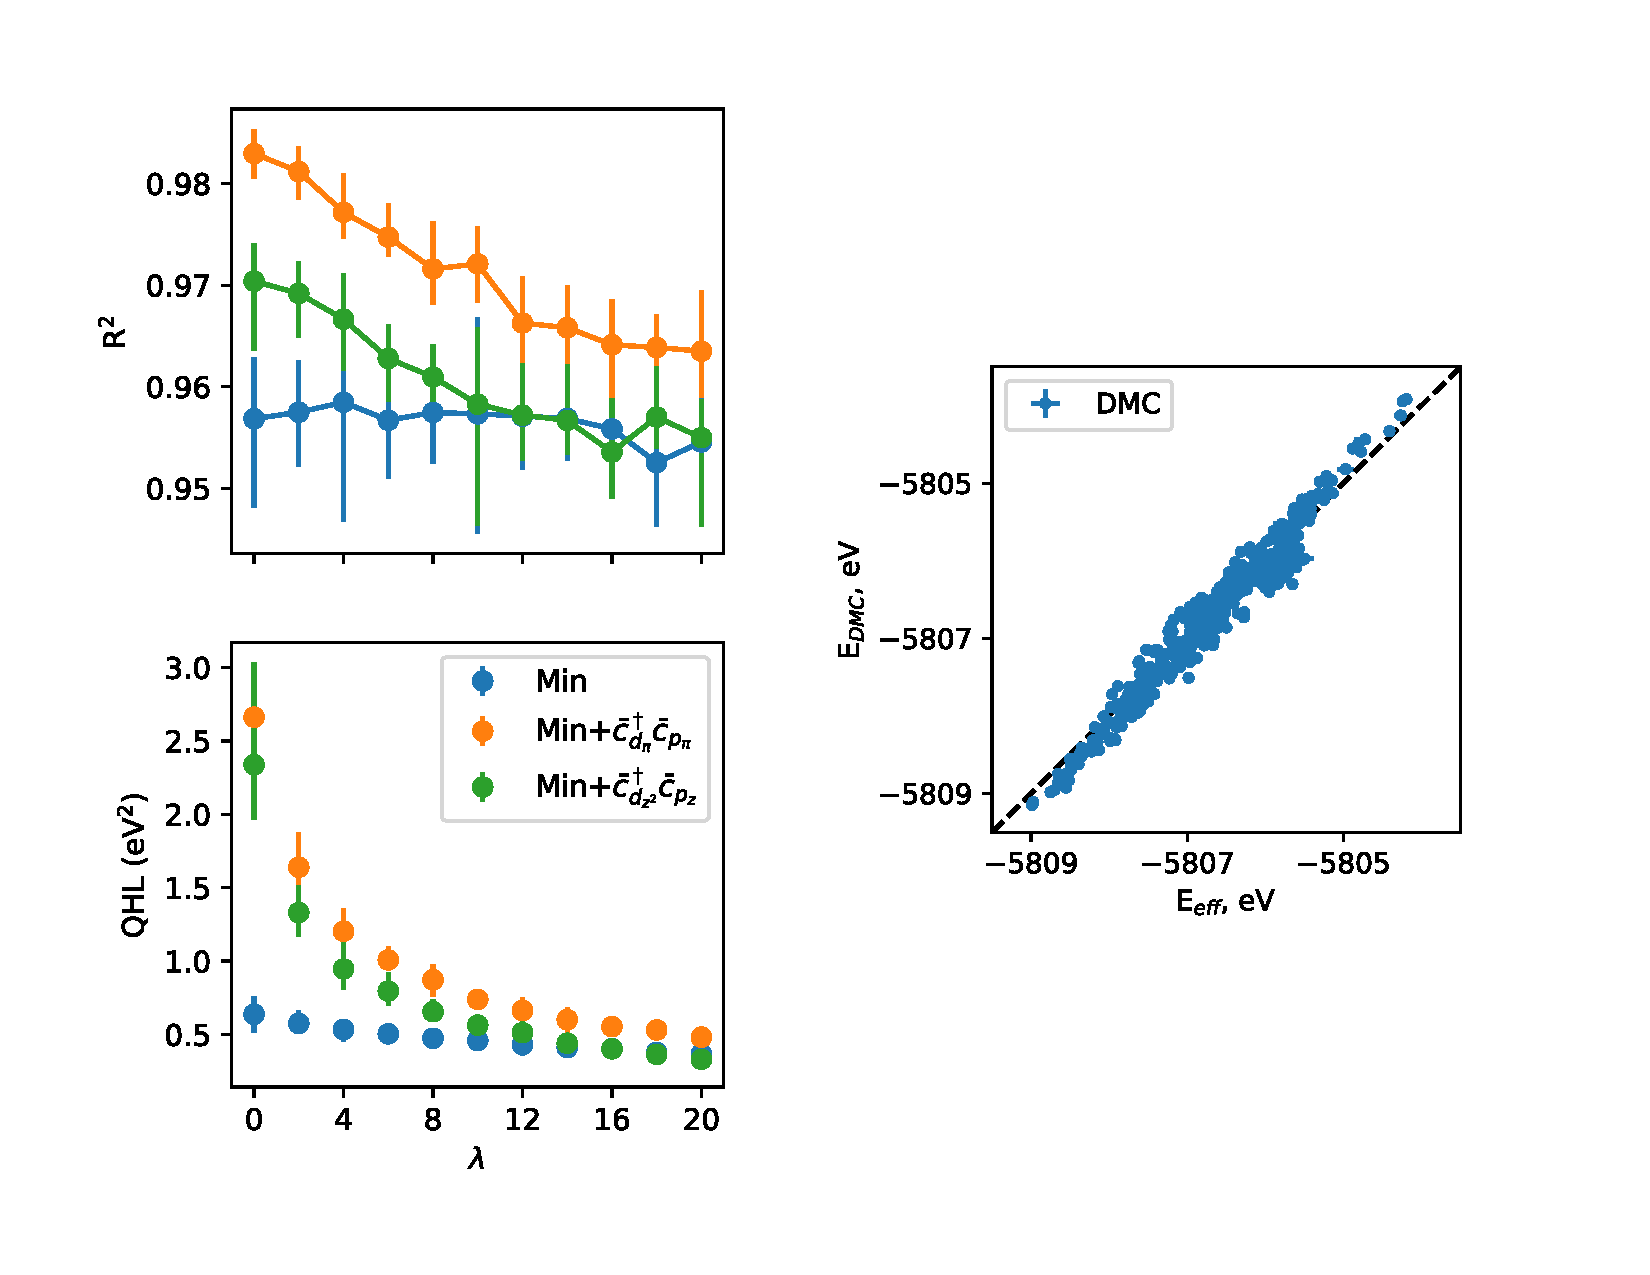
\includegraphics[width=0.7\linewidth]{../cuo/qwalk/old/ub3lyp_s1_/analysis/figs/prior_and_regr.pdf}
\end{center}
\caption{On the left, scores of the three candidate models at various $\lambda$ when fitting our effective theories using the cost function \eqref{eq:cost}. On the right we show predicted versus calculated energies for our low-energy sampled states for the minimal model fit at $\lambda = 20$.}
\label{fig:Prior}
\end{figure}

\begin{table}[H]
\begin{center}
\begin{tabular}{l|llllll}
&Min & Min & Min \\
& & $ + \bar{c}_{d_\pi}^\dagger \bar{c}_{p_\pi}$ & $ + \bar{c}_{d_{z^2}}^\dagger \bar{c}_{p_z}$ \\ $\ $ \\ \hline 
$\epsilon_{d_{z^2}}$& 0.32(2)& 0.32(1)& 0.29(2)\\
$\epsilon_{d_\pi}$& 0.19(1)& 0.10(2)& 0.19(1)\\
$\epsilon_{d_\delta}$& 0.0 & 0.0 & 0.0\\
$\epsilon_{4s}$& 2.2(4)& 2.23(3)& 2.19(5)\\
$\epsilon_{p_\pi}$& 1.7(3)& 1.8(2)& 1.7(3)\\
$\epsilon_{p_z}$& 0.96(4)& 0.97(3)& 0.99(5)\\
$t_\pi$& -0.57(1)& -0.45(2)& -0.57(1)\\
$t_{dz}$& 0.55(3)& 0.56(2)& 0.54(2)\\
$t_{sz}$& 0.87(2)& 0.89(2)& 0.85(2)\\
$t_{ds}$& 0.44(1)& 0.45(1)& 0.45(2)\\
$J_{sd}$& -0.6(1)& -0.8(1)& -0.6(1)\\
$U_s$& 3.8(2)& 3.7(2)& 3.9(2))\\
\end{tabular}
\\ $\ $
\\
\end{center}
Table 1: Parameters in eV for our three potential models when fit using \eqref{eq:cost} at $\lambda = 20$. Error bars are 95\% CI calculated using a bootstrap estimate.
\end{table}

\begin{figure}[H]
\centering
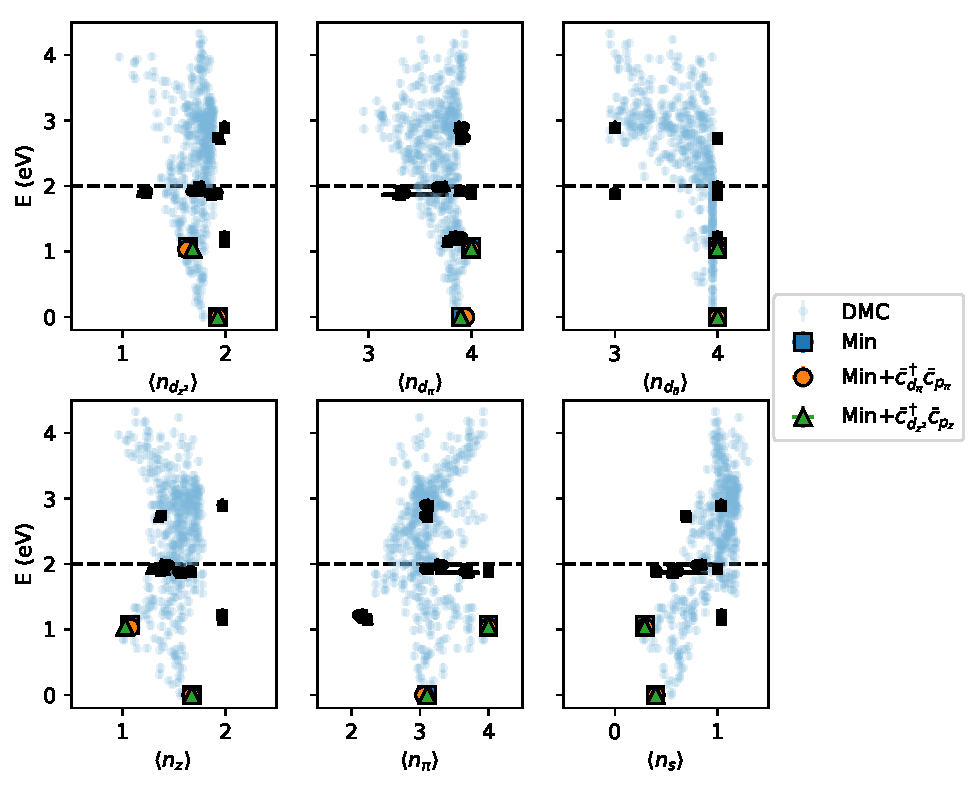
\includegraphics[width=0.7\linewidth]{../cuo/qwalk/old/ub3lyp_s1_/analysis/figs/final_ed.pdf}
\caption{Results of exact diagonalization showing the energies and properties of the first thirty eigenstates for three candidate models using linear regression with cost function \ref{eq:cost} and $\lambda = 20$. The ground state and first excited state are colored and have enlarged markers for clarity. Error bars are 95\% CI calculated by a bootstrap estimate.}
\label{fig:FinalED}
\end{figure}	

\section{Proposed work}
We want to develop low-energy effective theories for the
half-filled Hubbard model over the space U: 0 - 12, 1/k$_B$T: 0 - 3 using the DMD method, particularly focusing on the medium coupling region of U: 2 - 6 and 1/k$_B$T $\sim$ 1 where perturbative effective theories break down and a metal-insulator transition exists.
Similar to the case of the \textit{ab-initio} downfolding, we will need to construct low-energy spaces, sample the constructed spaces, build effective theories and respective bases, and fit our models.
Unlike \textit{ab-initio} downfolding, the Hubbard model downfolding has significantly fewer degrees of freedom, and therefore the DMD procedure can be done in a much more controlled fashion.
We will begin from a starting point of highest control, namely for system sizes small enough where we can exactly diagonalize the Hubbard model.
In the situation where we have full access to the eigenstates and spectra of a system, selecting $\mathcal{LE}$ can be done exactly as the span of some chosen $N$ lowest energy eigenstates. 
We can further guarantee that our sample set fully encapsulates all low-energy degrees of freedom by simply sampling states parameterized as $|\Psi\rangle = \sum_{j=1}^N c_j |\Phi_j\rangle$ where $|\Phi_j\rangle$ are eigenstates of the Hubbard Hamiltonian.
This can be seen in contrast to the CuO fitting where $\mathcal{LE}$ was defined implicitly through a number occupation descriptor and the sampling of $\mathcal{LE}$ was incomplete leading to intruder states in our initial effective theories.
Basis construction for the Hubbard Hamiltonian is also explicitly clear as any possible single particle basis we can use is just an orthogonal transformation of the basis the Hubbard model is defined on, and is guaranteed to be a complete single particle basis.
Again, this can be compared to the case of an \textit{ab-initio} system like the CuO molecule where bases are only approximately complete due to the huge number of degrees of freedom in the system.
In order to include temperature into the mix we can work with the full model Hilbert space such that $\mathcal{LE} = \mathcal{H}$, but generate samples within our space using a Monte Carlo sampling method according to a Boltzmann probability distribution with variable parameter $\beta = 1/k_BT$.
This way, our sample space will still be able to probe every excitation within a certain temperature range, the samples will be biased towards lower energy states according to the Boltzmann weight, and hence the fit model will also be biased towards describing more accurately the energy functional on the states with highest weight.
The Monte Carlo sampling may need to be altered further in order to deal with entropic effects when the density of states is very low in an energy range of interest and relatively high elsewhere.

Show in \ref{fig:Hubbard} is ... \textbf{SHOW OUR PRELIMINARY RESULTS}

In order to make any statements about effective theories for the Hubbard model we will have to work with larger system sizes and approximate methods like lattice quantum Monte Carlo to generate low-energy states for the DMD procedure. \textbf{TALK ABOUT FINITE SIZE SCALING AND APPROXIMATE METHODS (liken to FN-DMC for ab initio)}

A farther reaching goal would be to develop effective theories in the U-T-$\delta$ (doping) space for the Hubbard model, where more complex behavior similar to the cuprates superconductors have been found.

\end{document}